\chapter{Evaluation und Validation}
\label{ch:Eval}

\section{Vergleich mit Anforderungen}
\label{sec:VergleichAnforderungen}

\section{Fremde Wärmequellen}
\label{sec:FremdeWärmequellen}

In diesem Versuch wurde der Einfluss von fremden Wärmequellen wie zum Beispiel Laptops, Natels, oder Kaffees, Evaluiert. Dabei wurde der Effekt von Störquellen mit und ohne Personen im Raum analysiert.

\subsection{Resultate}
\label{subsec:FWresultate}

Der Threshold Algorithmus kann wie erwartet nicht gut mit anderen Wärmequellen umgehen. Dies weil der Threshold Algorithmus nur durch Temperatur und Mindestgrösse eines Objekts entscheiden Kann ob es sich um eine Person handelt. Deshalb hatte der Threshold Algorithmus auch eine nur eine Presicion score von \{Define\} erreicht.

Das CNN kann sehr gut mit anderen Wärmequellen umgehen, solange diese in ähnlicher Form antrainiert wurden. Da in einem Sitzungszimmer nicht viele unterschiedliche Wärmequellen vorkommen.

\vspace{.5em}
\begin{figure}[h!]
	\begin{subfigure}{.5\linewidth}
		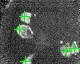
\includegraphics[keepaspectratio,height=4cm]{CNNDistance10}
		\caption{CNN Ergebnis des Distanztest mit 10cm Abstand}
		\label{fig:cnnDistance10}
	\end{subfigure}\hfill%
	\begin{subfigure}{.5\linewidth}
		\centering
		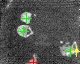
\includegraphics[keepaspectratio,height=4cm]{ThresholdDistance10}
		\caption{Threshold Ergebnis des Distanztest mit 10cm Abstand}
		\label{fig:thresholdDistance10}
	\end{subfigure}
	\begin{subfigure}{.8\linewidth}
		\centering
		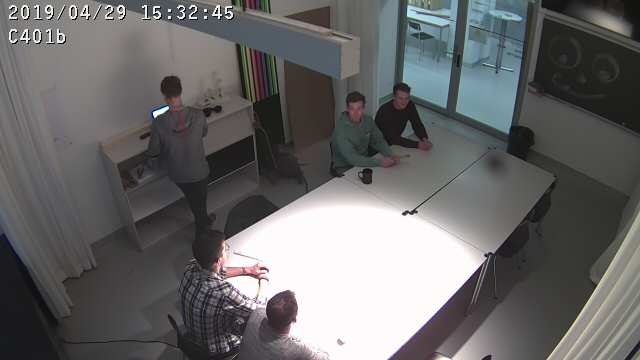
\includegraphics[keepaspectratio,height=3cm]{GroundDistance10}
		\caption{Ground-Truth}
		\label{fig:groundDistance10}
	\end{subfigure}
	\caption{Distanztest mit 10cm Abstand}
	\label{fig:versuchsaufbauten}
\end{figure}
\vspace{.5em}



\section{Distanz}
\label{sec:distanz}

Die Distanz zwischen zwei Personen ist ein wichtiger Faktor, der sich gleichermassen auf die Threshold-Methode auswirkt, wie auch auf das \gls{CNN}. Da bei dem \gls{CNN} mit einer Sliding-Window Methode und clustern der Treffer gearbeitet wird, kann das System bei Personen, welche zu wenig Abstand zueinander haben, nicht mehr zwischen den Treffern unterscheiden. Bei der Threshold-Methode wird die Silhouette der Personen leicht vergrössert, wodurch mehrere Personen bei geringem Abstand als einzelner Treffer gewertet werden.

\subsection{Resultate}

\textbf{\gls{CNN}}\\
Das \gls{CNN} kann Personen ab einem Abstand von 20cm auseinanderhalten, sofern diese sich im Zentrum des Bildes befinden. Um auf dem ganzen Bild fehlerfrei Personen zu erkennen müssen diese mindestens 40cm von Einander entfernt sein.

\textbf{Threshold}\\
Die Threshold-Methode erkennt Personen, im Zentrum des Bildes, ab einem Abstand von 10cm als einzelne Treffer. 

\begin{figure}[h!]
	\begin{subfigure}{.5\linewidth}
		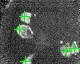
\includegraphics[keepaspectratio,height=4cm]{CNNDistance10}
		\caption{CNN Ergebnis des Distanztest mit 10cm Abstand}
		\label{fig:versuchaufbaunmr1}
	\end{subfigure}\hfill%
	\begin{subfigure}{.5\linewidth}
		\centering
		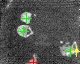
\includegraphics[keepaspectratio,height=4cm]{ThresholdDistance10}
		\caption{Threshold Ergebnis des Distanztest mit 10cm Abstand}
		\label{fig:versuchaufbaunmr7}
	\end{subfigure}
	\begin{subfigure}{.8\linewidth}
		\centering
		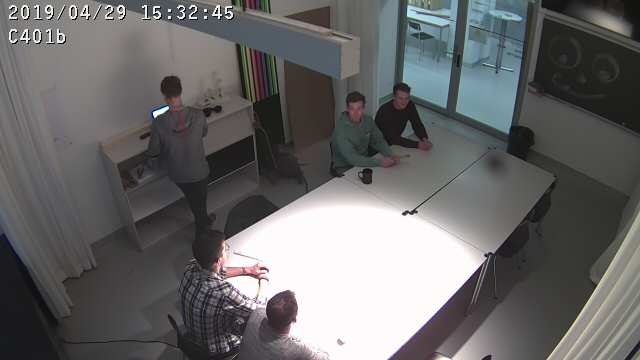
\includegraphics[keepaspectratio,height=4cm]{GroundDistance10}
		\caption{Ground-Truth}
		\label{fig:versuchaufbaunmr7}
	\end{subfigure}
	\caption{Zwei Versuchsaufbauten}
	\label{fig:versuchsaufbauten}
\end{figure}

\begin{figure}[h!]
	\begin{subfigure}{.5\linewidth}
		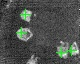
\includegraphics[keepaspectratio,height=4cm]{CNNDistance30}
		\caption{CNN Ergebnis des Distanztest mit 10cm Abstand}
		\label{fig:versuchaufbaunmr1}
	\end{subfigure}\hfill%
	\begin{subfigure}{.5\linewidth}
		\centering
		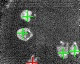
\includegraphics[keepaspectratio,height=4cm]{ThresholdDistance30}
		\caption{Threshold Ergebnis des Distanztest mit 10cm Abstand}
		\label{fig:versuchaufbaunmr7}
	\end{subfigure}
	\begin{subfigure}{.8\linewidth}
		\centering
		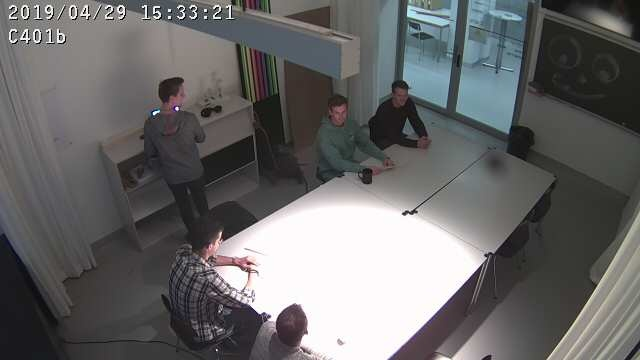
\includegraphics[keepaspectratio,height=4cm]{GroundDistance30}
		\caption{Ground-Truth}
		\label{fig:versuchaufbaunmr7}
	\end{subfigure}
	\caption{Zwei Versuchsaufbauten}
	\label{fig:versuchsaufbauten}
\end{figure}

